% Options for packages loaded elsewhere
\PassOptionsToPackage{unicode}{hyperref}
\PassOptionsToPackage{hyphens}{url}
%
\documentclass[
]{article}
\usepackage{lmodern}
\usepackage{amssymb,amsmath}
\usepackage{ifxetex,ifluatex}
\ifnum 0\ifxetex 1\fi\ifluatex 1\fi=0 % if pdftex
  \usepackage[T1]{fontenc}
  \usepackage[utf8]{inputenc}
  \usepackage{textcomp} % provide euro and other symbols
\else % if luatex or xetex
  \usepackage{unicode-math}
  \defaultfontfeatures{Scale=MatchLowercase}
  \defaultfontfeatures[\rmfamily]{Ligatures=TeX,Scale=1}
\fi
% Use upquote if available, for straight quotes in verbatim environments
\IfFileExists{upquote.sty}{\usepackage{upquote}}{}
\IfFileExists{microtype.sty}{% use microtype if available
  \usepackage[]{microtype}
  \UseMicrotypeSet[protrusion]{basicmath} % disable protrusion for tt fonts
}{}
\makeatletter
\@ifundefined{KOMAClassName}{% if non-KOMA class
  \IfFileExists{parskip.sty}{%
    \usepackage{parskip}
  }{% else
    \setlength{\parindent}{0pt}
    \setlength{\parskip}{6pt plus 2pt minus 1pt}}
}{% if KOMA class
  \KOMAoptions{parskip=half}}
\makeatother
\usepackage{xcolor}
\IfFileExists{xurl.sty}{\usepackage{xurl}}{} % add URL line breaks if available
\IfFileExists{bookmark.sty}{\usepackage{bookmark}}{\usepackage{hyperref}}
\hypersetup{
  pdftitle={FY20 Muskie Digital Campaign},
  pdfauthor={Office of Marketing and Brand Management},
  hidelinks,
  pdfcreator={LaTeX via pandoc}}
\urlstyle{same} % disable monospaced font for URLs
\usepackage[margin=1in]{geometry}
\usepackage{graphicx,grffile}
\makeatletter
\def\maxwidth{\ifdim\Gin@nat@width>\linewidth\linewidth\else\Gin@nat@width\fi}
\def\maxheight{\ifdim\Gin@nat@height>\textheight\textheight\else\Gin@nat@height\fi}
\makeatother
% Scale images if necessary, so that they will not overflow the page
% margins by default, and it is still possible to overwrite the defaults
% using explicit options in \includegraphics[width, height, ...]{}
\setkeys{Gin}{width=\maxwidth,height=\maxheight,keepaspectratio}
% Set default figure placement to htbp
\makeatletter
\def\fps@figure{htbp}
\makeatother
\setlength{\emergencystretch}{3em} % prevent overfull lines
\providecommand{\tightlist}{%
  \setlength{\itemsep}{0pt}\setlength{\parskip}{0pt}}
\setcounter{secnumdepth}{-\maxdimen} % remove section numbering
\usepackage{booktabs}
\usepackage{longtable}
\usepackage{array}
\usepackage{multirow}
\usepackage{wrapfig}
\usepackage{float}
\usepackage{colortbl}
\usepackage{pdflscape}
\usepackage{tabu}
\usepackage{threeparttable}
\usepackage{threeparttablex}
\usepackage[normalem]{ulem}
\usepackage{makecell}
\usepackage{xcolor}

\title{FY20 Muskie Digital Campaign}
\author{Office of Marketing and Brand Management}
\date{2/4/2020}

\begin{document}
\maketitle

Description:

The following report is a summary of the first 60 days of the Muskie
School's digital display advertising campaign. It started running on
November 27, 2019 and goes through the end of February.

The ads separately promote the MPH and the MPPM via 3 different
platforms; Facebook (FB), Programmatic (DBM), and LinkedIn (LI). This
report looks at performance data by program and vendor which is
illustrated by plots and tables. Benchmarks for the Click-through-Rates
(CTRs) are shown with a dotted black lines on the plots. The one record
table below each series of plots summarizes the metrics by the latest
week and the campaign to date.

\begin{verbatim}
## [1] "Note: Data updated 2020-02-11"
\end{verbatim}

\hypertarget{mph}{%
\subsection{MPH}\label{mph}}

\hypertarget{facebook-display}{%
\subsubsection{Facebook Display}\label{facebook-display}}

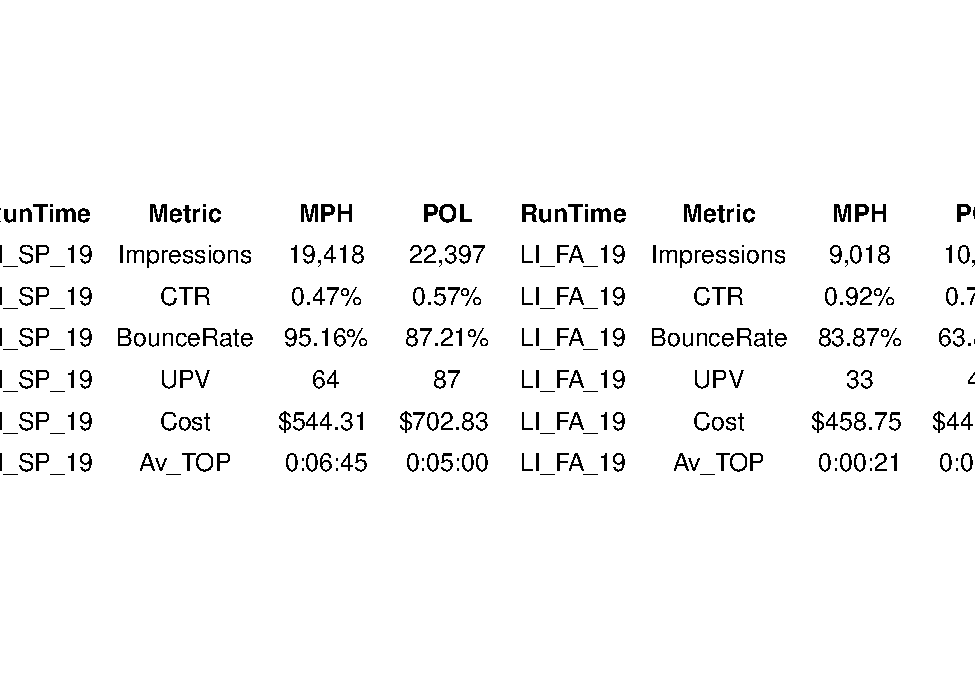
\includegraphics{Muskie_files/figure-latex/unnamed-chunk-4-1.pdf}

\begin{tabu} to \linewidth {>{\raggedleft}X>{\raggedright}X>{\raggedleft}X>{\raggedright}X>{\raggedleft}X>{\raggedright}X>{\raggedleft}X>{\raggedright}X}
\hline
\multicolumn{4}{c|}{This Week} & \multicolumn{4}{c}{Since Inception} \\
\cline{1-4} \cline{5-8}
Impressions & CTR & UPV & BR & YTD\_Imp & Avg\_CTR & YTD\_UPV & Avg\_BR\\
\hline
9630 & 0.17\% & 10 & 88.89\% & 236412 & 0.23\% & 357 & 90.53\%\\
\hline
\end{tabu}

\hypertarget{programmatic-display-display}{%
\subsubsection{Programmatic Display
Display}\label{programmatic-display-display}}

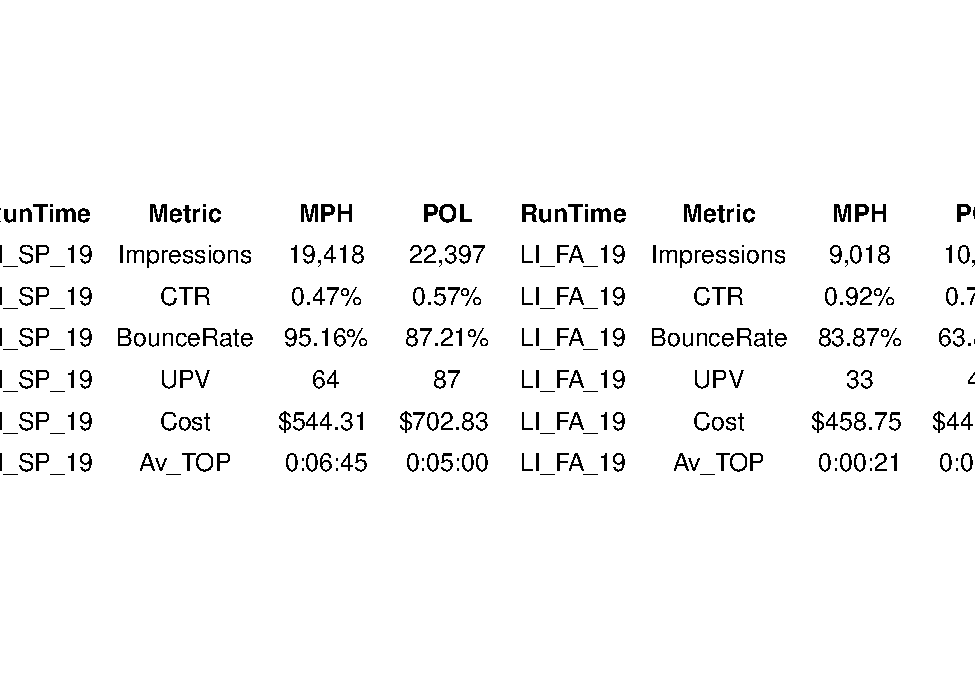
\includegraphics{Muskie_files/figure-latex/unnamed-chunk-5-1.pdf}

\begin{tabu} to \linewidth {>{\raggedleft}X>{\raggedright}X>{\raggedleft}X>{\raggedright}X>{\raggedleft}X>{\raggedright}X>{\raggedleft}X>{\raggedright}X}
\hline
\multicolumn{4}{c|}{This Week} & \multicolumn{4}{c}{Since Inception} \\
\cline{1-4} \cline{5-8}
Impressions & CTR & UPV & BR & YTD\_Imp & Avg\_CTR & YTD\_UPV & Avg\_BR\\
\hline
2822 & 0.35\% & 49 & 57.14\% & 82144 & 0.17\% & 483 & 57.71\%\\
\hline
\end{tabu}

\hypertarget{linkedin-sponsored-content}{%
\subsubsection{LinkedIn Sponsored
Content}\label{linkedin-sponsored-content}}

\includegraphics{Muskie_files/figure-latex/unnamed-chunk-6-1.pdf}

\begin{tabu} to \linewidth {>{\raggedleft}X>{\raggedright}X>{\raggedleft}X>{\raggedright}X>{\raggedleft}X>{\raggedright}X>{\raggedleft}X>{\raggedright}X}
\hline
\multicolumn{4}{c|}{This Week} & \multicolumn{4}{c}{Since Inception} \\
\cline{1-4} \cline{5-8}
Impressions & CTR & UPV & BR & YTD\_Imp & Avg\_CTR & YTD\_UPV & Avg\_BR\\
\hline
2183 & 0.64\% & 7 & 83.33\% & 23679 & 0.57\% & 61 & 93.33\%\\
\hline
\end{tabu}

\hypertarget{pol}{%
\subsection{POL}\label{pol}}

\hypertarget{facebook-display-1}{%
\subsubsection{Facebook Display}\label{facebook-display-1}}

\includegraphics{Muskie_files/figure-latex/unnamed-chunk-7-1.pdf}

\begin{tabu} to \linewidth {>{\raggedleft}X>{\raggedright}X>{\raggedleft}X>{\raggedright}X>{\raggedleft}X>{\raggedright}X>{\raggedleft}X>{\raggedright}X}
\hline
\multicolumn{4}{c|}{This Week} & \multicolumn{4}{c}{Since Inception} \\
\cline{1-4} \cline{5-8}
Impressions & CTR & UPV & BR & YTD\_Imp & Avg\_CTR & YTD\_UPV & Avg\_BR\\
\hline
10492 & 0.24\% & 16 & 100\% & 169163 & 0.3\% & 283 & 91.57\%\\
\hline
\end{tabu}

\hypertarget{programmatic-display-display-1}{%
\subsubsection{Programmatic Display
Display}\label{programmatic-display-display-1}}

\includegraphics{Muskie_files/figure-latex/unnamed-chunk-8-1.pdf}

\begin{tabu} to \linewidth {>{\raggedleft}X>{\raggedright}X>{\raggedleft}X>{\raggedright}X>{\raggedleft}X>{\raggedright}X>{\raggedleft}X>{\raggedright}X}
\hline
\multicolumn{4}{c|}{This Week} & \multicolumn{4}{c}{Since Inception} \\
\cline{1-4} \cline{5-8}
Impressions & CTR & UPV & BR & YTD\_Imp & Avg\_CTR & YTD\_UPV & Avg\_BR\\
\hline
2897 & 0.31\% & 41 & 60.98\% & 83057 & 0.2\% & 498 & 57.76\%\\
\hline
\end{tabu}

\hypertarget{linkedin-sponsored-content-1}{%
\subsubsection{LinkedIn Sponsored
Content}\label{linkedin-sponsored-content-1}}

\includegraphics{Muskie_files/figure-latex/unnamed-chunk-9-1.pdf}

\begin{tabu} to \linewidth {>{\raggedleft}X>{\raggedright}X>{\raggedleft}X>{\raggedright}X>{\raggedleft}X>{\raggedright}X>{\raggedleft}X>{\raggedright}X}
\hline
\multicolumn{4}{c|}{This Week} & \multicolumn{4}{c}{Since Inception} \\
\cline{1-4} \cline{5-8}
Impressions & CTR & UPV & BR & YTD\_Imp & Avg\_CTR & YTD\_UPV & Avg\_BR\\
\hline
2162 & 0.56\% & 16 & 86.67\% & 25307 & 0.58\% & 137 & 83.19\%\\
\hline
\end{tabu}

\hypertarget{conclusions}{%
\section{Conclusions:}\label{conclusions}}

\begin{itemize}
\item
  From an ad performance perspective, DBM and LI are doing well with
  CTRs above the USM and National benchmarks respectively.
\item
  DBM and FB drive the most traffic and DBM has a very good bounce rate.
\end{itemize}

\end{document}
